%!TEX root = /Users/andy/Documents/Academics/Dissertation/thesis.tex

\begin{savequote}[75mm] 
Motor behaviors are built out of a sequence of movements that evolve through time. From the most basic, such as locomotion,the the most complex, such as playing the piano,t he timing of movements is crucial.
\qauthor{Michael A. Long and Michale S. Fee, \citep{long_using_2008}} 
\end{savequote}

\chapter{Bending waves during \textit{Caenorhabditis elegans} locomotion are driven and organized by proprioceptive coupling }\label{chapter:proprioceptive}


\section{Introduction}
\lettrine{H}{ow neural circuits give rise to coordinated rhythmic behaviors} such as locomotion remains a fundamental question in systems neuroscience 
\citep{delcomyn_neural_1980}. Classic studies sought the neuromuscular 
basis of locomotion in aquatic swimmers such as lamprey and leech \citep{marder_principles_1996,kristan_rhythmic_1976,cohen_neuronal_1980,friesen_neuronal_1978,ermentrout_frequency_1984}. In these systems, the concept of a Central Pattern Generator (CPG) is commonly evoked to explain rhythmic behavior \citep{delcomyn_neural_1980,marder_principles_1996}. The CPG hypothesis is supported by observations that motor neurons in each body segment continue to exhibit rhythmic activity even after pruning all inputs \citep{kristan_rhythmic_1976,cohen_neuronal_1980,pearce_intersegmental_1984}.




Whereas a CPG could produce rhythmic behavior, motor circuits still need to respond to sensory 
inputs to deliver precise and flexible control of body movement \citep{delcomyn_neural_1980}. In leech, muscle activity can be coordinated among segments by sensory feedback even after cutting neuronal couplings between segments \citep{yu_sensory_1999}. In \textit{Drosophila} larva, specific classes of mechanosensory neurons that tile the body contribute to organizing peristaltic waves during locomotion \citep{hughes_sensory_2007,song_peripheral_2007,cheng_role_2010}. In \textit{C. 
elegans}, the shape and speed of bending waves adapt to the mechanical load imposed by the 
environment \citep{fang-yen_biomechanical_2010,berri_forward_2009}, and mutations in a mechanosensitive channel (TRP-4) acting in the DVA 
interneuron perturb the amplitude and frequency of body undulation \citep{li_c._2006}.


Here, we sought a biophysical characterization of the role of proprioceptive feedback in the \textit{C. elegans} locomotory circuit by combining microfluidics and optical neurophysiology \citep{liewald_optogenetic_2008,chronis_microfluidics_2007,zhang_multimodal_2007,clark_temporal_2007,lockery_artificial_2008}. We discovered that stretch-sensitive coupling between adjacent body regions represents the key mechanism for driving bending waves along the worm body during forward locomotion.





\section{Results}
\subsection{The bending of one body region requires the bending of its anterior neighbor}

\textit{C. elegans} moves forward by propagating dorsal-ventral body bending waves from head to tail. 
The detailed kinematics of bending waves can be quantified using the time-varying curvature 
measured at each point along the body centerline over time (Fig.~\ref{fig:prop1}a). To compare data from different worms, we normalized distance along the centerline by measuring fractional distance 
from head to tail (head $=0$; tail $=1$). Each body region alternates between positive (red) and 
negative (blue) curvature, and bands of curvature propagate from head to tail as shown in a 
kymograph (Fig.~\ref{fig:prop1}b). 




\begin{FPfigure} 
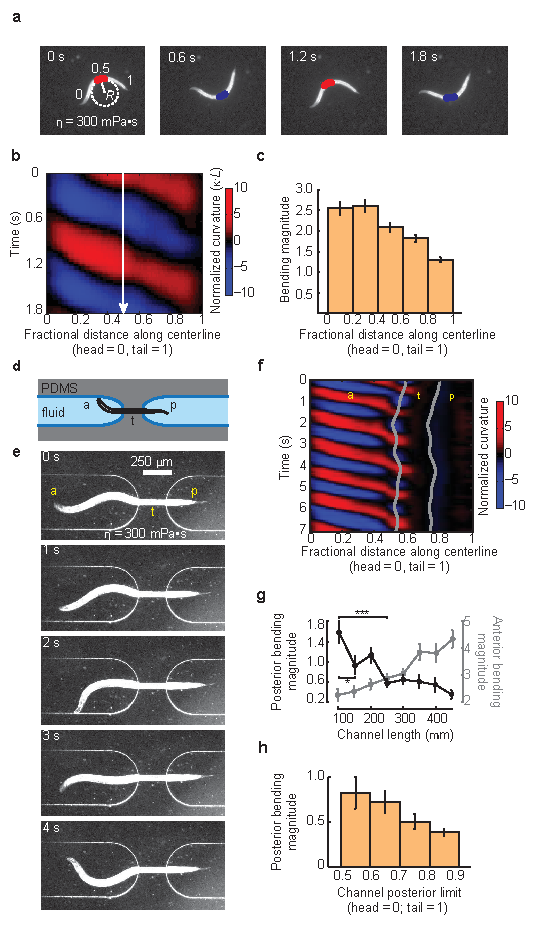
\includegraphics[width=\textwidth]{figures/prop1}
\caption[Bending of posterior regions requires anterior bending. ] {Bending of posterior regions requires anterior bending. (\textbf{a}) Video images of a worm swimming forward. Bending is quantified by measuring the radius 	of curvature R at each point along the centerline. Position along the centerline is measured in normalized coordinates using the fractional distance from head to tail (head $= 0$; tail $= 1$). A red-blue colormap illustrates alternating curvatures at fractional distance $= 0.5$. (\textbf{b}) Kymograph of time-varying curvature illustrating retrograde bending waves along the worm represented in non-dimensional units. To do this, the curvature at each point along the centerline, $\kappa = 1/R$, is multiplied by worm length, $L$. (\textbf{c}) Bending magnitude along the body of a wide-type free swimming worm, measured as the standard deviation of normalized curvature over time. $n = 18$ worms, mean $\pm$ one standard error. (\textbf{d}) Schematic of microfluidic device. a stands for anterior region, p stands for posterior region, and t stands for trapped region of a worm.  (\textbf{e}) Video images of a wide-type young adult worm exhibiting forward undulatory gait inside the microfluidic device (also see Video  \ref{video:prop1}). The channel divides the worm body into unrestrained anterior, posterior, and trapped middle regions. (\textbf{f}) Kymograph of time-varying curvature along the body of the worm shown in (\textbf{e}). Gray lines mark the anterior and posterior limits of the straight channel. (\textbf{g}) Bending magnitude of a posterior and an anterior body region (\textasciitilde$0.15$ worm length) adjacent to the channel, measured as the standard deviation of time-varying normalized curvature, is plotted as a function of the length of the trapped region. $n \geq 10$ worms for each condition, mean  $15$	$\pm$ one standard error. Position of the posterior limit of the channel is $0.7 \pm 0.1$ (mean $\pm$ standard deviation) for each condition, measured as the fractional distance from head to tail. *$P<0.05$, ***$P = 0.0001$, Mann-Whitney U test.  (\textbf{h}) Bending magnitude of a posterior body region (mean $\pm$ one standard error) as a function of the position of the posterior limit of the channel. We measured 64 bouts of forward movement trapped in different channel positions from $20$ worms. Channel length is $300 \mu$m.\label{fig:prop1}}
\end{FPfigure}
\afterpage{\clearpage}



First, we sought to determine whether the motor activity in one body region depends on the 
bending of neighboring body regions. To test this, we designed microfluidic devices that enabled 
us to immobilize body regions of varying length along the middle of a young adult worm (Fig.~\ref{fig:prop1}d-e and Video \ref{video:prop1}). Our first device trapped the center of a worm in a narrow 
straight channel. The region of the worm's body inside the channel was restrained, while  regions of the worm's body either anterior or 
posterior to the channel were free to bend (Fig.~\ref{fig:prop1}d-e). We used a channel diameter ($40 \mu$m) that was sufficient to 
immobilize the trapped region (worm diameter is $54 \pm 4 \mu$m; mean $\pm$ SD) with minimum 
constriction.  

We consistently recorded bouts of forward movement ($> 10$ s) when we set the posterior limit of 
the channel at $0.7 \pm 0.1$ in fractional worm length along the body. Bending waves would 
propagate normally to the anterior limit of the channel (gray data points in Fig.~\ref{fig:prop1}g). Short 
channels ($100 \mu$m long) did not affect wave propagation along the worm body; the bending wave 
that emerged from the posterior limit of the channel (black data points in Fig.~\ref{fig:prop1}g) exhibited 
similar amplitude as a free swimming worm (Fig.~\ref{fig:prop1}c). However, increasing channel length 
beyond $200 \mu$m significantly diminished the bending amplitude in the posterior body region (Fig.~\ref{fig:prop1}e-g). Fixing the channel length, but moving it toward the tail also reduced the posterior 
bending amplitude (Fig.~\ref{fig:prop1}h, $R = -0.24$, $p < 0.05$, Spearman’s rank correlation test).

To determine whether immobilization directly affects muscle activity in body regions within and 
posterior to the channel, we quantified intracellular calcium dynamics in the muscle cells of 
transgenic worms (P\textit{myo3::G-CaMP3::RFP}) expressing the calcium indicator G-CaMP3 \citep{tian_imaging_2009} and RFP in all body wall muscles (Supplementary Fig.~\ref{fig:prop_sup2} and Video \ref{video:prop2}). While 
muscle cells anterior to the channel exhibited strong rhythmic intracellular calcium dynamics 
during the propagation of bending waves, muscle cells within and posterior to the channel had 
much lower levels of calcium dynamics (Supplementary Fig.~\ref{fig:prop_sup2}).

Taken together, these results suggest that immobilizing a body region lowers motor activity 
within and posterior to that region, thereby disrupting bending wave propagation. Motor activity 
in one body region seems to require active bending of anterior regions extending \textasciitilde200 \textmu m.

\subsection{Muscle activity is positively correlated with the curvature of adjacent anterior 
neighbors}
 
To further explore how the bending of adjacent body regions is coupled, we designed 
microfluidic devices that trapped the middle region of a worm at defined curvatures (Fig.~\ref{fig:prop2}a,c). 
Here, we used channels that were at least $250 \mu$m long to prevent bending waves from 
propagating into the unrestrained posterior part. The unrestrained posterior region exhibited 
static curvature in the same direction as that imposed on the middle region trapped by the 
channel (Fig.~\ref{fig:prop2}a-b and Video  \ref{video:prop3}). By using channels with different curvatures, we 
found that the curvature of the posterior region increased linearly with the imposed curvature on 
the trapped middle region with slope $0.62 \pm 0.03 L$ (Fig.~\ref{fig:prop2}d). 



\begin{FPfigure} 
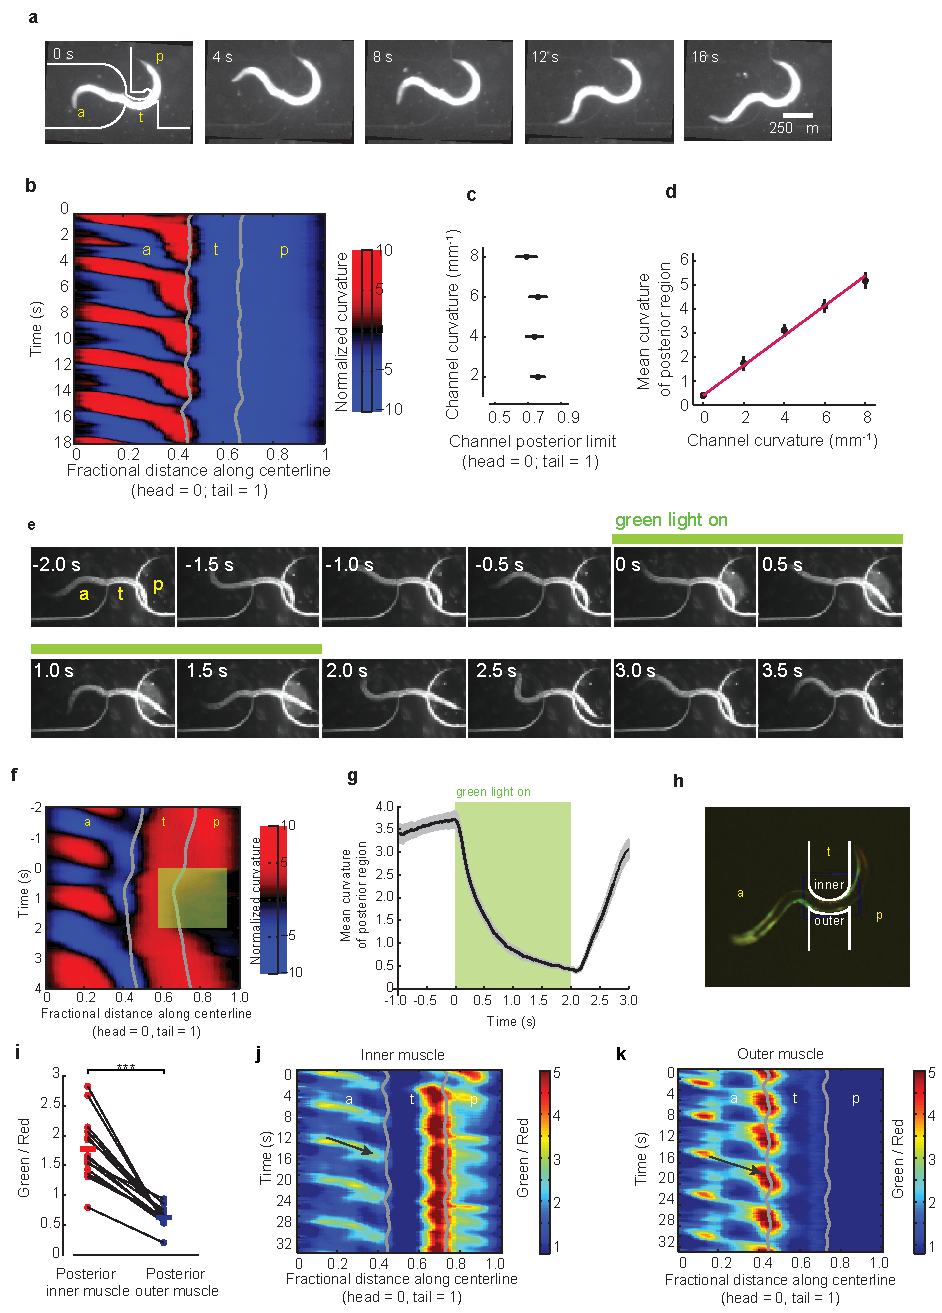
\includegraphics[width=\textwidth]{figures/prop2}
\caption[Bending of posterior regions is positively correlated with anterior bending. ] {Bending of posterior regions is positively correlated with anterior bending. (\textbf{a}) Video images of a worm exhibiting forward undulatory gait while partially constrained in a 
curved microfluidic channel (also see Video  \ref{video:prop3}). 
(\textbf{b}) Kymograph of normalized curvature of the worm shown in (\textbf{a}). Gray lines show anterior and 
posterior limits of the curved channel. 
(\textbf{c}) Positions of the posterior limit of the curved channel (mean $\pm$ standard deviation). $n \geq 8$ 
worms for each condition,  
(\textbf{d}) The curvature of the unrestrained posterior body region, measured as a spatial average from 
the posterior limit of the channel to the tail and a temporal average over bouts of forward 
movement, is plotted as a function of channel curvature. Each data point (mean $\pm$ one standard 
error) represents data from at least 8 animals. Magenta line is the linear least square fit of the 
data with a slope $0.62 \pm 0.03~L$.  
(\textbf{e}) Video images of a transgenic worm (P\textit{myo3::NpHR}) partially constrained in a curved 
microfluidic channel. The green bar indicates a $2$ s interval during which the posterior body 
region emerging from the channel was illuminated by green light (also see Video  \ref{video:prop4}). 
(\textbf{f}) Kymograph of normalized curvature of the animal shown in (\textbf{e}). Green shading indicates the 
body region and duration of green light illumination.  
(\textbf{g}) Mean curvature $\pm$ one standard error of the posterior region emerging from the curved 
channels as shown in (\textbf{a}) during green light illumination (\textasciitilde$30$ measurements using 6 worms). 
(\textbf{h}) Calcium imaging of body wall muscles in a partially constrained transgenic worm 
(P\textit{myo3::G-CaMP3::RFP}) in a curved channel. Red fluorescence from RFP constitutes the 
reference signal. Green fluorescence from G-CaMP3 indicates intracellular calcium levels. The 
contours of the microfluidic channel are drawn in white (also see Video  \ref{video:prop5}). 
(\textbf{i}) Comparison of the ratio of green fluorescence to red fluorescence intensity emitted from inner 
and outer muscles of the posterior body region. Each data point represents a spatial average of 
the ratio over a posterior body region (\textasciitilde$0.2$ worm length) adjacent to the channel and a temporal 
average over a bout of forward movement. Solid lines indicate population mean. Among $14$ 
measurements from six worms, six measurements restrict dorsal muscles on the inner side. ***$P= 0.00001$, Mann-Whitney U test. 
(\textbf{j,k}) Representative ratiometric kymograph of calcium levels in inner (\textbf{j}) and outer (\textbf{k}) muscle 
cells of a worm trapped in the device shown in (\textbf{h}). Higher/lower ratios of green fluorescence to 
red fluorescence in each set of body wall muscles indicate higher/lower intracellular calcium 
levels. Arrows highlight one calcium wave that propagates from the head to the anterior limit of 
the curved channel along the inner musculature (\textbf{j}) and outer musculature (\textbf{k}).\label{fig:prop2}}
\end{FPfigure}
\afterpage{\clearpage}


We sought to verify that the static curvature of the posterior unrestrained region was driven by 
muscle activity, and not through passive mechanical properties of the worm body. First, we used 
transgenic worms (\textit{Pmyo3::NpHR}) that express halorhodopsin \citep{han_multiple-color_2007} in all body wall muscles. 
When we induced muscle relaxation in the unrestrained posterior region with green light, we 
found that the tail reversibly straightened during illumination (Fig.~\ref{fig:prop2}e-g and 
Video \ref{video:prop4}). Second, we directly monitored muscle activity in the curved posterior region using 
 $5$
transgenic worms (P\textit{myo3::G-CaMP3::RFP}) that expressed both G-CaMP3 and RFP in all body 
wall muscle cells (Fig.~\ref{fig:prop2}h). Using this strain, intracellular calcium levels within a cell can be 
inferred from the ratio of green to red fluorescence--the higher the ratio, the higher the 
intracellular calcium concentration. In the posterior region emerging from the channel, we 
consistently measured higher calcium levels in the muscle cells on the inner side than the outer 
side of the curved body (Fig.~\ref{fig:prop2}i-k). Third, when the whole animal was paralyzed with sodium 
azide, the body regions emerging from the curved channel remained straight (Video \ref{video:prop6}). These experiments suggest that the static curvature of the posterior unrestrained region 
is due to a fixed pattern of motor circuit activity. 


Taken together, our results suggest that proprioceptive coupling contributes to propagating the 
bending signal along the worm body during forward movement. Through positive stretch-sensitive feedback, posterior regions are compelled to bend in the same direction and in 
proportion to the bending of adjacent anterior regions. 
 
\subsection{Post-channel body curvature follows channel curvature with a viscosity- 
dependent delay}
 
To characterize the temporal dynamics of proprioceptive coupling, we measured the time lag 
between the bending in one body region and the induced bending in the neighboring posterior 
region. To do this, we designed pneumatic microfluidic devices to rapidly change the curvature 
of one region of a worm. We flanked both sides of a thin channel with two independently 
controllable inflatable chambers (Fig.~\ref{fig:prop3}a). By simultaneously pressurizing one chamber while 
depressurizing the other, we were able to induce rapid curvature changes in a specific region of a 
trapped worm. 

\begin{FPfigure} 
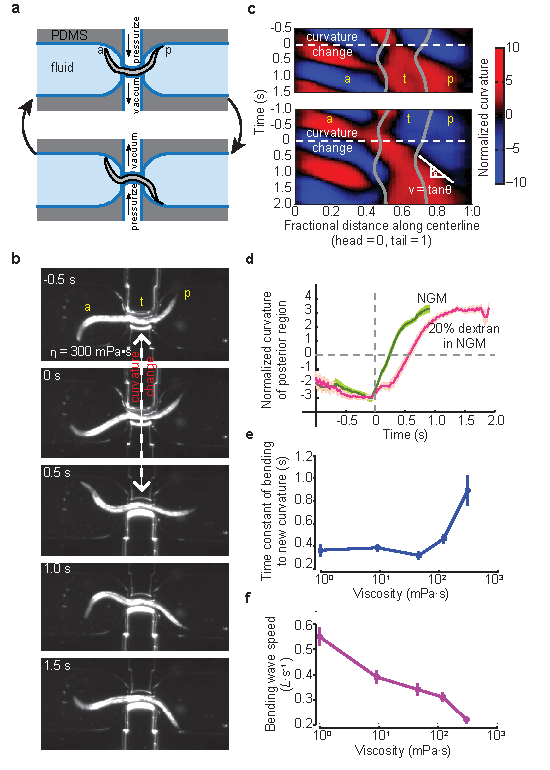
\includegraphics[width=\textwidth]{figures/prop3}
\caption[Pneumatic microfluidic device for manipulating body curvature.] {Pneumatic microfluidic device for manipulating body curvature.  
(\textbf{a}) Schematic of the pneumatic microfluidic device. The channel is flanked by two chambers. By 
alternatively pressurizing one chamber while depressurizing the other, the curvature of a region 
of a trapped worm is rapidly switched. 
(\textbf{b}) Video images of a partially immobilized wild-type worm. At $t = 0$ s, the channel starts to 
change its curvature (also see Video  \ref{video:prop7}). 
(\textbf{c}) Two representative curvature kymographs of a worm trapped in the pneumatic channel. Gray 
lines mark the anterior and posterior limits of the curved channels. White dashed lines at $t = 0$ s 
mark the induced change in channel curvature from negative (color blue) to positive (color red). 
While the unrestricted anterior body region exhibits opposite bending activities in the two 
kymographs, this difference did not affect the dynamics of the induced curvature change in the 
unrestricted posterior body region. The bending wave that shifts the posterior region from 
negative to positive curvature propagates with velocity equal to the slope of the zero crossing in 
curvature (color black) as shown. 

(\textbf{d}) The time course of curvature change in the immediate posterior region (\textasciitilde$0.1$ worm length) 
emerging from the pneumatic channel after the switch of channel curvature at $t = 0$ s. The two 
curves correspond to experiments conducted in two different viscosities (NGM buffer and $20\%$ 
dextran in NGM). Error bars indicate one standard error.  
(\textbf{e}) The time constant for relaxation of the posterior region to new curvatures obtained by fitting 
exponentials to time courses as shown in (\textbf{d}). Each data point represents at least $30$ 
measurements from five worms. Error bars indicate $95\%$ confidence interval to the exponential 
fits.  
(\textbf{f}) The speed of the bending wave following induced changes in channel curvature as a function 
of fluid viscosity. Error bars indicate one standard error.\label{fig:prop3}}
\end{FPfigure}
\afterpage{\clearpage}


As with the static curved channels, we found that the curvature of the worm body posterior to the 
dynamic channel was positively correlated with channel curvature. Switching channel curvature 
to either side induced a switch in the curvature of the posterior body region (Fig.~\ref{fig:prop3}b-c and 
Video  \ref{video:prop7}). This result also underscores dorsal-ventral symmetry in the coupling 
mechanism between adjacent body regions. 

We found that the switch in curvature of the posterior unrestrained region propagated with 
measurable speed from the posterior limit of the channel to the tail, consistent with the flow of a 
retrograde bending signal (Fig.~\ref{fig:prop3}c-f). We sought to determine whether the delayed bending of the 
posterior region represented mechanical damping by the external viscous fluid and/or internal 
delays within the neuromuscular network. To do this, we studied worms that were immersed in 
fluids of different viscosity (Fig.~\ref{fig:prop3}d-f). We found that the bending delay was roughly constant, 
\textasciitilde300 ms, in fluids ranging from 1 mPa·s (the viscosity of water) to \textasciitilde100 mPa·s. In more viscous 
fluids, the bending delay began to increase, becoming \textasciitilde1 s at $300$ mPa·s. These results suggest 
that \textasciitilde300 ms represents an upper bound for delays within the neuromuscular network, which 
become rate-limiting at low viscosities. Interestingly, \textasciitilde300 ms also coincides with the undulation 
period for \textit{C. elegans} swimming in water, and may represent the time constant that sets the 
upper limit to undulation frequency. Delays within the neuromuscular network might reflect 
signaling delays in synaptic transmission and/or the limiting speed of muscle contraction.

\subsection{Stretch-sensitive feedback requires cholinergic motor neurons }
 
Cholinergic motor neurons that innervate the ventral and dorsal muscle cells are required for \textit{C. elegans} locomotion \citep{chalfie_neural_1985,leifer_optogenetic_2011}. B-type cholinergic motor neurons are required for forward 
locomotion, whereas A-type cholinergic motor neurons are required for backward movement 
\citep{chalfie_neural_1985}. We asked whether the cholinergic neurons  play a role in the proprioceptive coupling  that propagates the bending signal along the worm body. First, we trapped transgenic worms 
(P\textit{unc17::NpHR}) that expressed halorhodopsin in all cholinergic motor neurons in the pneumatic 
microfluidic devices and illuminated them with green light. We found that deactivating the 
cholinergic neurons prevented posterior body regions from following induced changes in 
the curvature of the anterior region (Fig.~\ref{fig:prop4} and Video  \ref{video:prop8}). Instead, optogenetic 
inactivation of the cholinergic neurons arrests the worm in the posture immediately preceding 
green light illumination.  


\begin{figure} 
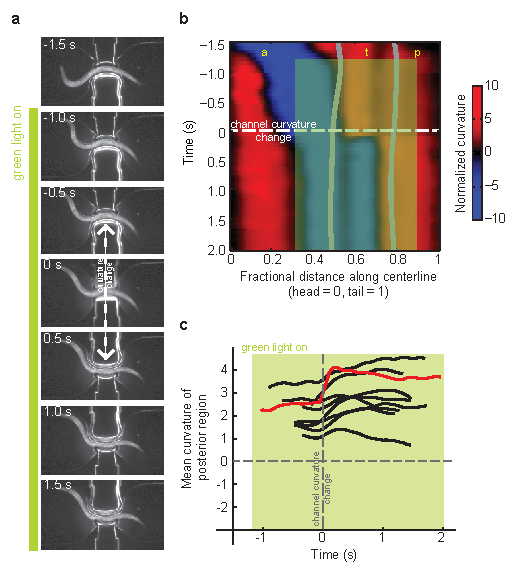
\includegraphics[width=0.87\textwidth]{figures/prop4}
\caption[ Optogenetic inactivation of cholinergic motor neurons.] { Optogenetic inactivation of cholinergic motor neurons.   
(\textbf{a}) Video images of a transgenic worm (P\textit{unc17::NpHR}) partially trapped in a pneumatic 
microfluidic channel. Green bar indicates the duration of green light illumination of the middle 
portion of the worm before and after induced change in channel curvature at $t = 0$ s. As a result, 
the curvature of the tail failed to follow the curvature change of the channel (also see 
Video  \ref{video:prop8}). 
(\textbf{b}) Curvature kymograph of the transgenic worm trapped in the channel as shown in (\textbf{a}). Green 
shading indicates the body region and duration of green light illumination. 
(\textbf{c}) Curvature of the posterior body region, measured as an average from the posterior limit of the 
channel to the tail, during onset of illumination (green shading) and the induced change in 
curvature of the middle region at $t = 0$ (dashed line). Representative data from five worms were 
shown. Red curve corresponds to the experiment shown in (\textbf{a}) and (\textbf{b}). 
\label{fig:prop4}}
\end{figure}

Next, we studied \textit{vab-7} mutants, whose dorsal B-type cholinergic motor neurons (DB) reverse 
the direction of their processes \citep{esmaeili_c._2002}. During unrestrained forward movement, the bending wave 
in the anterior of \textit{vab-7} mutants exhibits both dorsal and ventral curvatures, whereas the bending 
wave that propagates to posterior regions exhibits only ventral curvatures (Supplementary Fig.~\ref{fig:prop_sup3}a, c-d and Video  \ref{video:prop9}). In other words, only ventral bending waves propagate 
through the worm body. When we trapped \textit{vab-7} mutants in the pneumatic microfluidic device, 
we found that the posterior region of the worm was unable to follow the bending of the channel 
to the dorsal side (Supplementary Fig.~\ref{fig:prop_sup3}b, e-f and Video  \ref{video:prop10}). Taken together, 
these results suggest that the B-type cholinergic motor neurons are required to close a 
proprioceptive feedback loop that drives the bending signal along the motor circuit during 
forward movement. 


\subsection{Body wall muscles exhibit hysteresis}
 
Deactivating cholinergic motor neurons in transgenic worms (P\textit{unc17::NpHR}) locked the worm 
in whatever bending posture the worm had adopted immediately preceding illumination (Fig. ~\ref{fig:prop4} and  \citep{leifer_optogenetic_2011}). Accordingly, we ask 
whether \textit{C. elegans} muscles can sustain contraction even in the absence of motor neuron inputs. 

To test this possibility, we optogenetically stimulated body segments in transgenic worms (P\textit{myo- 3::ChR2}) expressing Channelrhodopsin-2 in body wall muscles while eliminating motor neuron 
inputs. To remove motor neuron inputs, we treated transgenic worms with ivermectin, which 
hyperpolarizes the motor circuit by activating glutamate gated chloride channels \citep{dent_genetics_2000,cully_cloning_1994}, but 
does not directly affect muscle cells \citep{hart_behavior_2006}. When we optogenetically induced body bending in 
paralyzed worms, the bend would persist long after turning off the illumination (Supplementary Fig.~\ref{fig:prop_sup4}a-b and Video  \ref{video:prop11}). The bend would gradually relax over \textasciitilde40 s, but often in 
a series of abrupt jumps (Supplementary Fig.~\ref{fig:prop_sup4}c). We observed similar a phenomenon when 
ivermectin treated worms are in the \textit{unc-13(s69)} background (Video  \ref{video:prop12}), a loss 
of function mutation that prevents synaptic transmission from both GABAergic and cholinergic 
motor neurons to muscles \citep{richmond_unc-13_1999}. Taken together, these results suggest that \textit{C. elegans} body wall 
muscles indeed exhibit a form of hysteresis: they can maintain stable levels of contraction long after stimulation.  

\section{Discussion}
Russell and Byerly noted that the cholinergic motor neurons have long and synapse-free 
processes that extend along the ventral and dorsal nerve cords. They speculated that these 
processes might represent stretch-sensitive antennae to detect changes in body posture (cited in 
 \citep{white_structure_1986,chen_neuronal_2007} and Supplementary Fig.~\ref{fig:prop_sup1}b). In theoretical models of the worm motor circuit, 
Niebur and Erdos \citep{niebur_theory_1991} used proprioceptive coupling hypotheses as a mechanism to propagate 
bending signals. Here, we have shown that cholinergic motor neurons are required to 
transduce stretch-sensitive signals, and that this form of proprioceptive coupling represents a key 
mechanism for propagating bending signals along the \textit{C. elegans} body during forward 
locomotion. Posterior body segments are compelled to bend in the same direction as anterior 
segments through stretch-sensitive signals transduced by cholinergic motor neurons. 
Proprioceptive coupling could explain the organization of the undulatory gait without the need to 
invoke ensembles of center pattern generators (CPG) along the motor circuit, like body segments 
in lamprey and leech are thought to behave \citep{ermentrout_frequency_1984}.  
 
The small size and experimental accessibility of the \textit{C. elegans} motor circuit suggest that it might 
be possible to build computational models of locomotion that integrate the dynamics of all 
neuronal and muscle components. Our results suggest that any computational framework for the 
\textit{C. elegans} locomotory circuit must integrate the biomechanics of undulatory movement itself 
with neuromuscular activity. In \textit{C. elegans}, the motor circuit organizes the undulatory gait for forward locomotion by both detecting and driving bending activity.


\section{Material and Methods} 
 
\subsection{Worm strains} 
Wild-type worms (N2 Bristol) were cultivated at 20 \textdegree C using standard methods. 
We performed all experiments using young adult worms within a few hours after their final molt. 
The \textit{vab-7} mutant strain was obtained from the \textit{C. elegans} Genetics Center (Minneapolis, MN, US). The \textit{unc-13(s69)} mutant strain was a gift from E. Jorgensen. 
 
Transgenic worms carrying extrachromosomal arrays (P\textit{myo3::G-CaMP3:RFP}) were used for 
calcium imaging in body wall muscle activities. The promoter sequence of the P\textit{myo-3} gene \citep{kuroyanagi_transgenic_2006} and the coding sequences of \textit{GCaMP3} and tagRFP-T were ligated to the pSM backbone. The \textit{G-CaMP3} and \textit{tagRFP-T} sequences were separated by a SL2 trans-splicing site. The construct was 
injected into N2 worms to obtain extrachromosomal arrays.  

The transgenic worms used in all optogenetic experiments were cultivated in the dark at 20 \textdegree C on 
NGM plates with Escherichia coli OP50 and all-trans retinal. We made OP50-retinal plates by 
seeding each 6-cm NGM plate with 250 $\mu$l OP50 and 1 $\mu$l 100 mM retinal in ethanol. Strains used are ZX444 [\textit{lin-15}(n765ts); \textit{zxEx29} (P\textit{myo-3::NpHR::ECFP}; \textit{lin-15+})] , ZM 5016 \textit{hpls178} [P\textit{unc-17::NpHR::ECFP}] and ZM5398 \textit{hpls199}[\textit{Pmyo3::ChR2::EGFP}] . ZX444 was a gift from A. Gottschalk and the extrachromosomal array was integrated by cobalt-60 irradiation and outcrossing three times to wild-type worm. Strains ZM 5016 and ZM5398 were gifts from M. Zhen. The strain \textit{unc-13}(s69); \textit{hpls199}[P\textit{myo3::ChR2::EGFP}] was made by crossing \textit{unc-13}(s69) with \textit{hpls199}. 

\subsection{Microfluidic devices} 
Microfluidic devices were fabricated using standard soft lithography. Each 
design was drawn in Clewin and sent to a laser-printing service (CAD/Art Services, Inc. Bandon, 
OR).  A master was created by patterning features of SU-8 negative photoresist (Microchem 
Corp., Newton, MA, US) on a silicon wafer using photolithography. This master was then used 
to mold microfluidic channels in PDMS. To facilitate the release of the PDMS device from the 
master, we treated the master with vapor of tridecafluoro(1,1,2,2 tetrahydroooctyl) 
trichlorosilane (Gelest, Inc., Philadelphia, PA, US) inside a vacuum chamber. The PDMS 
prepolymer was mixed with Sylgard 184, its curing agent, at specific weight ratios (20:1 for the 
 10
pneumatic microfluidic device and 10:1 for other devices). After pouring the PDMS prepolymer 
over the master, we cured the PDMS at 60 \textdegree C for 8 h and peeled the PDMS slab from the master. 
A circular biopsy punch (1.5 mm in diameter, Shoney Scientific Inc., Waukesha, WI, US) was used to 
create inlets and outlets for the microfluidic channels. The PDMS slab was bonded to a glass 
coverslip by treating the surfaces of the glass and the PDMS slab with air plasma for two 
minutes and 30 s respectively. The PDMS was bonded to another PDMS slab in the 
pneumatic microfludic device.


We loaded the microfluidic channel with NGM buffer or dextran solution [\textasciitilde 20\\% dextran in NGM (wt/vol) in most cases]. An individual worm was flowed into the inlet of each microfluidic 
channel and worm position within each channel was manually controlled by syringes connected 
to polyethylene tubing (1.57 mm outer diameter and 1.22 mm inner diameter). In the calcium 
imaging experiments, channel depth was \textasciitilde 38 \textmu m. In all other cases, channel depth was \textasciitilde 85 \textmu m. 
In the pneumatic microfluidic device, the channel was flanked by two chambers that could be 
alternatively pressurized and depressurized with a valve system under computer control using 
custom software written in LabVIEW (National Instruments, Austin, TX, US). 


\subsection{Measuring locomotion of partially immobilized worms}

Experiments were performed on 
Nikon microscopes (TE2000 or Eclipse LV150) under 4X magnification with dark field 
illumination. Image sequences were taken by a CCD camera (Imaging Source) and recorded on a 
computer at 30 Hz using IC Capture software (Imaging Source).  
 
Image analysis was performed using custom  software written in MATLAB (MathWorks, Inc. 
Natick, MA, US) following methods described in \citep{fang-yen_biomechanical_2010}. Briefly, we identified image sequences in 
which the worm persistently exhibited its forward undulatory gait, i.e., bending waves 
propagated backward from the head. After background subtraction to eliminate features of the 
microfluidic channel, we filtered and thresholded each image to obtain a binary image. The head 
and tail were identified as the points of maximum convex curvature on the worm boundary. A 
centerline extending from the head to the tail of the worm was calculated so that each point is 
roughly equidistant to nearest boundary points on two sides of the animal. The centerline was 
then fit by a least-squares cubic smoothing spline. Curvature, by definition, was calculated as the 
magnitude of the derivative of the unit vector tangent to the centerline with respect to the body 
coordinate along the centerline. In the experiment using pneumatic microfludic devices, the 
speed of the bending wave of the body region posterior to the channel was calculated using least-square linear fits to the zero crossings of curvature (Fig.~\ref{fig:prop4}c). 



\subsection{Ivermectin-induced paralysis.}
Young adult transgenic worms (\textit{hpls199} [\textit{Pmyo3::ChR2::EGFP}] 
or \textit{unc-13}; \textit{hpls199}) were placed in ivermectin solution (0.02 mg/mL in NGM) sandwiched 
between two glass sides separated by 127 \textmu m. Worms were free to swim until completely 
paralyzed after \textasciitilde 30 min, when they were used for optogenetic stimulation.

\subsection{Calcium imaging of body wall muscle activities.}

GCaMP3 and RFP were excited by LEDs 
filtered at 448-492nm and 554-572nm respectively using Semrock single-bandpass filters. 
Fluorescence emission was recorded through an Olympus MVX Plan Apochromat 2X objective 
(working distance 20mm, numerical aperture 0.5). The fluorescence image was split by a Cairns 
Optosplit II Image Splitter and the two images (green channel, 499-525 nm; red channel, 581- 
619 nm) were projected onto two halves of an Andor iXon 885 EMCCD camera. A DinoLite Pro 
AM413T USB camera was used to track the worm using Worm Tracker 2.0 software developed 
by the Schafer lab. Zaber T-LSR075A Motorized Linear Slides give automated x-y stage 
movement. Imaging sequences were recorded on a computer at 10 Hz using Andor Solis 
software and converted into TIFF files using ImageJ. Images were then analyzed using custom-written MATLAB scripts. Briefly, the two split images were re-aligned and the calcium activities 
of muscles were calculated as the ratio of green to red fluorescence emission intensities. The true 
emission intensities from the two channels were calculated using the following formulas: True 
green = green measured – green background; True red = red measured – red background – 
0.153*True green. There is 15.3\% bleedthrough from the green to the red channel. 

\subsection{Optogenetic stimulation.}
 We used two optical setups to stimulate transgenic worms expressing 
Channelrhodopsin (ChR2) or Halorhodopsin (Halo). Experiments with the pneumatic 
microfluidic device were conducted on a Nikon microscope (Eclipse LV150) under 10X 
magnification with dark field illumination. A mercury arc lamp with green filter and field 
 12
diaphragm was used to illuminate the worm with controlled spot size. Rhodamine in the 
microfluidic channel (10 \textmu M) allowed us to directly visualize the area and duration of green light 
illumination. 
Other optogenetic experiments were conducted on a modified version of the CoLBeRT system, 
described in \citep{leifer_optogenetic_2011}. Briefly, the CoLBeRT system consists of an inverted Nikon microscope 
(TE2000), blue and green diode pumped solid state lasers, a high speed CCD camera, and a 
digital micromirror device all under the control of the open source MindControl software. Each worm 
was imaged under red light with dark field illumination, and the digital micromirror device 
reflected laser light to shine on targeted cells or regions of the worm. For the \textit{unc-13}; 
P\textit{myo3::ChR2} and ivermectin-treated worm experiments, the CoLBeRT system was modified to 
programmatically control laser intensity. To do this, the MindControl software interfaces with 
custom-written LabVIEW software that modulates the analog voltage signal sent to the laser 
power controllers via a LabJack U3-HV digital-to-analog converter. MindControl and associated software is available at \url{http://github.com/samuellab}.  

\section{Accompanying Video}
\subsection{Video 1}\label{video:prop1}
 
A young adult N2 worm was swimming forward in dextran solution [20\% dextran in NGM 
(wt/vol)] while the middle region of its body was constrained in a straight microfluidic channel. 
Body undulation can propagate to the anterior limit of the channel, but bending waves emerging 
from the posterior limit of the channel were hardly detected and the unrestricted posterior body 
region remained straight (QuickTime; 12.2 MB). 
 
\subsection{Video 2}\label{video:prop2}
 
A young adult transgenic worm expressing calcium indicators in body wall muscle cells 
(P\textit{myo3::G-CaMP3::RFP}) was swimming forward in dextran solution [15\% dextran in NGM] 
while the middle region of its body was constrained in a straight microfluidic channel. White 
lines show the boundary of the channel. Pseudo-color shows the ratio of green fluorescence 
(emitted from G-CaMP3) to red fluorescence (from RFP). Higher ratio, which indicates higher 
calcium activities, is represented by a larger value of the red component in the muscle color map. 
Muscle cells within and posterior to the channel had lower levels of intracellular calcium 
dynamics than muscle cells anterior to the channel that drove bending waves (QuickTime; 0.56 
MB).   
 
\subsection{Video 3 }\label{video:prop3}
 
A young adult N2 worm was swimming forward in dextran solution (20\% dextran in NGM) 
while the middle region of its body was constrained in a curved microfluidic channel. The 
unrestricted posterior region of the worm exhibited static curvature in the same direction as 
that imposed on the middle region by the channel (QuickTime; 0.82 MB). 
 
\subsection{Video 4 }\label{video:prop4}
 
A young adult transgenic worm  expressing halorhodopsin in its body wall muscles 
(Pmyo3::NpHR) was swimming forward in dextran solution (20\% dextran in NGM) while the 
middle region of its body was constrained in a curved microfluidic channel. A bright circular spot 
appeared when the posterior body region was illuminated by green light. During illumination, the 
unstrained posterior body region was reversibly straightened (QuickTime; 1.6 MB). 
 
\subsection{Video 5 }\label{video:prop5}
 
A young adult transgenic worm that expresses calcium indicators in body wall muscle cells 
(P\textit{myo3::G-CaMP3::RFP}) was swimming forward in dextran solution (15\% dextran in NGM) 
while the middle region of its body was constrained in a curved microfluidic channel. White 
lines show the boundary of the channel. Pseudo-color shows the ratio of green fluorescence 
(from G-CaMP3) to red fluorescence (from RFP). Higher ratio is represented by a larger value of 
the red component in the muscle color map. During forward locomotion, the muscle cells at the 
inner side of the posterior body region emerging from the channel consistently exhibited higher 
calcium activities than the outer side (QuickTime; 5.5 MB). 
 
\subsection{Video 6}\label{video:prop6}
 
After being fully paralyzed by sodium azide, a young adult N2 worm was partially constrained in a 
curved pneumatic microfluidic channel. The unrestrained body regions emerged from the 
channel always remained straight (QuickTime; 0.46 MB).    
 
\subsection{Video 7}\label{video:prop7}
 
Young adult N2 worms were moving forward while the middle regions of their bodies were 
constrained in pneumatic microfluidic channels. In the first half of the video, a worm was 
swimming forward in NGM buffer solution. Switching the bending direction of the channel 
quickly induced the switch in the bending direction of the posterior body region. In the second 
half of the video, a worm was swimming forward in more viscous fluid (20\% dextran solution in 
NGM). In this case, there was a more significant delay between switching the bending of the 
channel and switching the bending direction in the posterior body region (QuickTime; 5.7 MB). 
 
\subsection{Video 8}\label{video:prop8} 
 
A young adult transgenic worm (P\textit{unc17::NpHR}) that expressed halorhodopsin in all cholinergic 
motor neurons was moving forward while the middle region of the body was constrained in an 
pneumatic microfluidic channel. During green light illumination, the unrestrained posterior body 
region failed to follow the switch of channel curvature (QuickTime; 1.7 MB). 
 
\subsection{Video 9}\label{video:prop9}
 
A young adult \textit{vab-7} mutant was moving freely in 20\% dextran solution. The ventral and dorsal 
side of the worm can be identified by the location of eggs from the dark field illumination. 
During forward locomotion, dorsal bending waves could not propagate throughout the body and the 
posterior body region always curved ventrally (QuickTime; 1.3 MB). 
 
\subsection{Video 10} \label{video:prop10}
 
A young adult \textit{vab-7} mutant was moving forward while the middle region of its body was 
constrained in an inflatable microfluidic channel. Bending the channel to the dorsal side failed to 
induce the switch in the bending direction of the posterior body region (QuickTime; 1.2 MB). 
 
\subsection{Video 11}\label{video:prop11}
 
This video shows 2 s blue light illumination of an ivermectin-treated paralyzed 
transgenic worm (P\textit{myo3::ChR2}) that expressed Channelrhodopsin-2 in body wall muscles. 
When DLP was on, blue light illuminated a rectangular region near the middle of the worm and 
induced body bending. When DLP was off, there was no light stimulation but the bending 
persisted for a long period (QuickTime; 3.8 MB). 
 
 

\subsection{Video 12}\label{video:prop12}
 
This video shows 2 s blue light illumination of an ivermectin-treated paralyzed 
transgenic worm (P\textit{myo3::ChR2}) in the \textit{unc-13}(s69) background. When DLP was on, blue light 
illuminated a rectangular region near the middle of the worm and induced body bending. When 
DLP was off, there was no light stimulation but the bending persisted for a long period. 


\section{Supplementary Materials}
\subsection{Parallels to songbird motor pathway}
The work presented here tries to address previously open questions about how the sequential activation of muscles in \textit{C. elegans} is coordinated and controlled and what role muscles, motorneurons and feedback play, respectively. Prior to this work,  existing data was insufficient to discriminate between conflicting models. For example, in one model  sequential activation of motorneurons  could  drive muscle contraction without any proprioceptive feedback. In another model, muscles could propagate  bending waves by sequentially activating neighboring muscles via gap junctions without any need for proprioceptive feedback and with motorneurons playing only a modulatory role. Yet other models suggested that proprioceptive feedback was the driving force behind wave propagation, which is in fact consistent with the observations shown here.

By selectively inhibiting regions of muscles, motorneurons and physical restraining different regions of the worms body, this work rules  supports a model based on proprioceptive feedback. Namely, motorneurons are thought to be activated by yet-to-be discovered stretch sensors which in turn drive muscles in one region to contract, which in turn activate stretch sensors,  which finally induce posterior motorneurons to contract---  perpetuating a cycle that propagates bending waves.

The questions posed and the experimental approach taken in this work has parallels to prior work done by Michael Long and Michale Fee studying birdsong in zebra finch \citep{long_using_2008}. In that work, Long and Fee were interested in similar types of questions related to songbird motor pathway. They asked what role interneurons in a brain region HVC and motorneurons in a region RA played, respectively, in sequential muscle activation required for birdsong. Prior to their work, it was hypothesized that HVC sequentially initiated small subsequences of shorter time-scale motor activation that were handled entirely within RA. By selectively cooling either RA or HVC and observing slowing in the resulting birdsong they show that HVC directly induces each motorneuron activation in RA, even on short time scales. 
They also show that  two independent hemispheres of HVC take turns controlling the motor sequence and they provide evidence that feedback downstream of RA is used to keep the two hemispheres synchronized. 

Both works use selective inactivation of different subcircuits to explore the temporal dependence of sequential activation of motor activity. Both works also point to the importance of feedback from downstream areas back to high level interneurons and motoneurons in coordinating complex motor sequences.  Together these two works pave the way for future experiments exploring motor sequence generation in further detail.

\begin{FPfigure} 
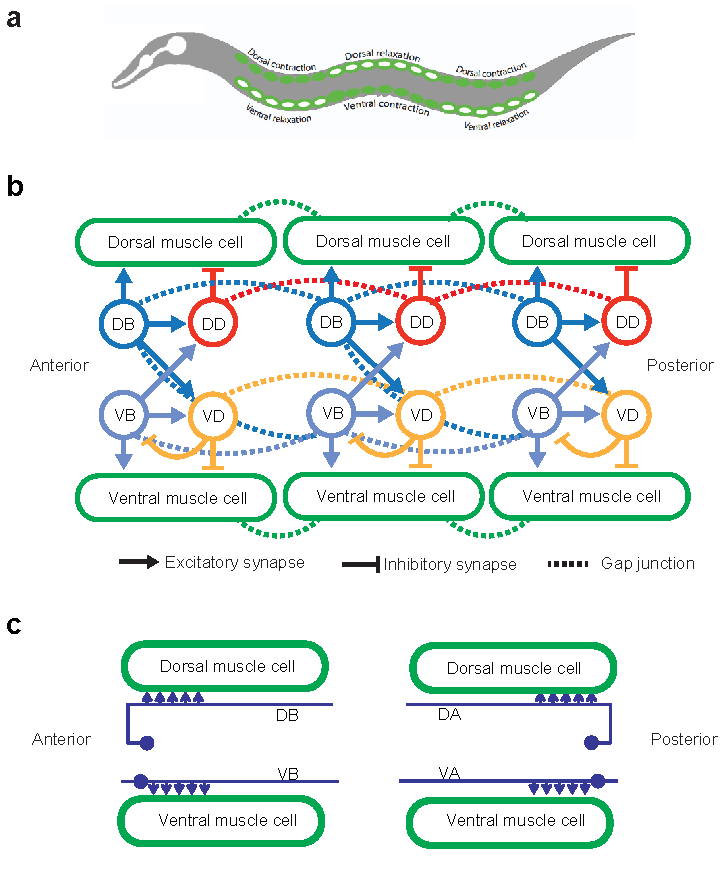
\includegraphics{figures/prop_sup1}
\caption[Schematic of the motor circuit in C. elegans.] { Schematic of the motor circuit in C. elegans. 
(\textbf{a}) Worms undulate by alternating contraction and relaxation of dorsal and ventral muscle cells lining 
the body. Dorsal bending is achieved when dorsal muscle cells contract (filled cells) and ventral muscle 
cells relax (open cells). Ventral bending is achieved when ventral muscle cells contract and dorsal 
muscle cells relax. 
(\textbf{b}) General patterns of connectivity in the wiring diagram for forward movement adapted from \citep{hughes_sensory_2007,song_peripheral_2007} . 
Arrows indicate excitatory chemical synapses from the cholinergic motor neurons (VB and DB, in light and dark blue, respectively). Blunt ended 
lines indicate inhibitory chemical synapses from GABAergic motor neurons (DD and VD, in red and orange, respectively). GABAergic neurons 
are dispensable for the propagation of the bending wave along the worm body. Dashed lines indicate gap 
junctions between neighboring muscle cells and neighboring neurons of each cell type. Six to twelve neurons 
of each cell type are distributed along the worm body. 
  
(\textbf{c}) Schematic of the morphology of B-type cholinergic motoneurons that are required for forward movement 
and A-type cholinergic motor neurons that are required for backward movement. Arrows indicate synapses, 
circles represent somas and lines indicate the direction and path of neuronal processes. B-type motor neurons 
extend long processes without synapses in the posterior direction. A-type motor neurons extend long processes 
without synapses in the anterior direction (adapted from \citep{chen_neuronal_2007}). 
\label{fig:prop_sup1}}
\end{FPfigure}

\begin{FPfigure} 
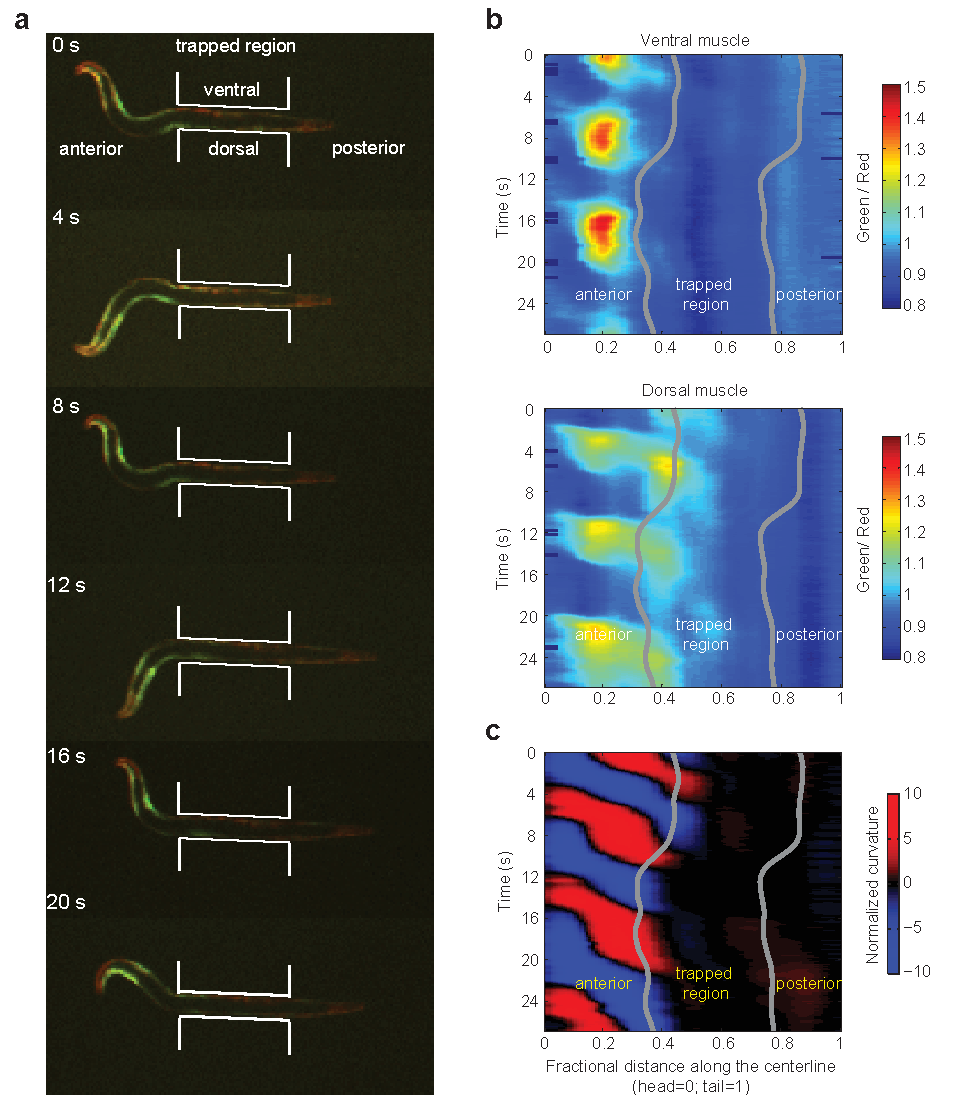
\includegraphics[width=\textwidth]{figures/prop_sup2}
\caption[Intracellular calcium dynamics in muscle cells.] { Intracellular calcium dynamics in muscle cells of a transgenic 
worm (P\textit{myo3::G-CaMP3::RFP}) partially constrained in a straight microfluidic channel. 
 
(\textbf{a}) Video images of a worm exhibiting forward locomotory gait while partially immobilized in a straight 
microfluidic channel. Red fluorescence constitutes the reference channel emanating from RFP in the 
muscle cells. Green fluorescence constitutes the calcium-sensitive signal emanating from GCaMP3. 
White lines show the boundary of the channel (also see Video  \ref{video:prop2}). 
(\textbf{b}) Ratiometric analysis of intracellular calcium dynamics within the ventral and dorsal muscle cells 
of the worm trapped in the straight channel shown in (\textbf{a}). Higher ratios of green to red fluorescence 
indicate higher intracellular calcium levels. Intracellular calcium levels in both the ventral (upper 
kymograph) and dorsal muscles (lower kymograph) of the posterior region emerging from the straight 
channel are lower than in the anterior region. Representative result from one of the five worms studied. 
(\textbf{c}) Kymograph of time-varying body curvature for the worm trapped in the straight channel shown in (\textbf{a}). 
\label{fig:prop_sup2}}
\end{FPfigure}

\begin{FPfigure} 
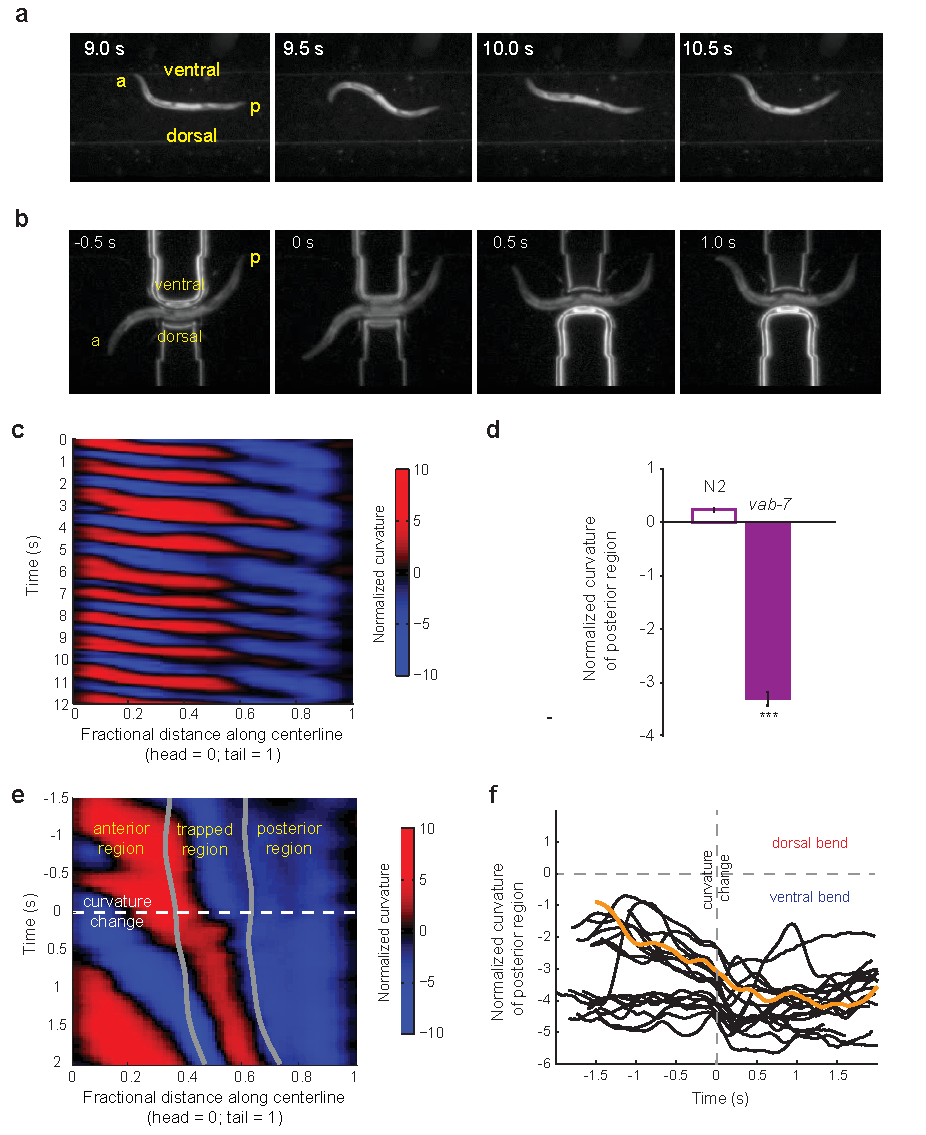
\includegraphics[width=\textwidth]{figures/prop_sup3}
\caption[\textit{vab-7} mutants.] { Undulatory wave propagation disrupted in \textit{vab-7} mutants. 
(\textbf{a,b}) Video images of a \textit{vab-7} mutant worm freely swimming in water (\textbf{a}) and trapped 
in a pneumatic microfluidic device (\textbf{b}). Ventral and dorsal side of the worm are distinguished 
by using the eggs as markers. 
(\textbf{c}) Kymograph of a freely swimming \textit{vab-7} mutant worm show bending waves propagate 
from head to tail. Anterior regions alternate between dorsal curvature (red) and ventral 
curvature (blue). Posterior regions alternate between null curvature (black) and ventral 
curvature (blue) (also see Video  \ref{video:prop9}). (\textbf{d})  Curvature of the posterior body 
region (0.6-0.8 body length), average over an integer number of undulation periods, 
in a free swimming worm. $n ≥ 6$ for each data point. ***$p = 0.0002$, Mann-Whitney U test. 
(\textbf{e}) Kymograph of \textit{vab-7} mutant worm trapped in the pneumatic microfluidic device as 
shown in (\textbf{b}). Changing the curvature of the trapped middle region towards the dorsal 
side (red) does not induce dorsal curvature in the posterior region (also see Supplemental 
Video 10). (\textbf{f}) Curvature of the posterior body region, measured as an average from the 
posterior limit of the channel to the tail, before and after the induced curvature change in the 
trapped middle region at $t = 0$. Representative trials from six worms. Orange curve 
corresponds to the experiment shown in (\textbf{b}) and (\textbf{e}).   
\label{fig:prop_sup3}}
\end{FPfigure}
\afterpage{\clearpage}


\begin{figure} 
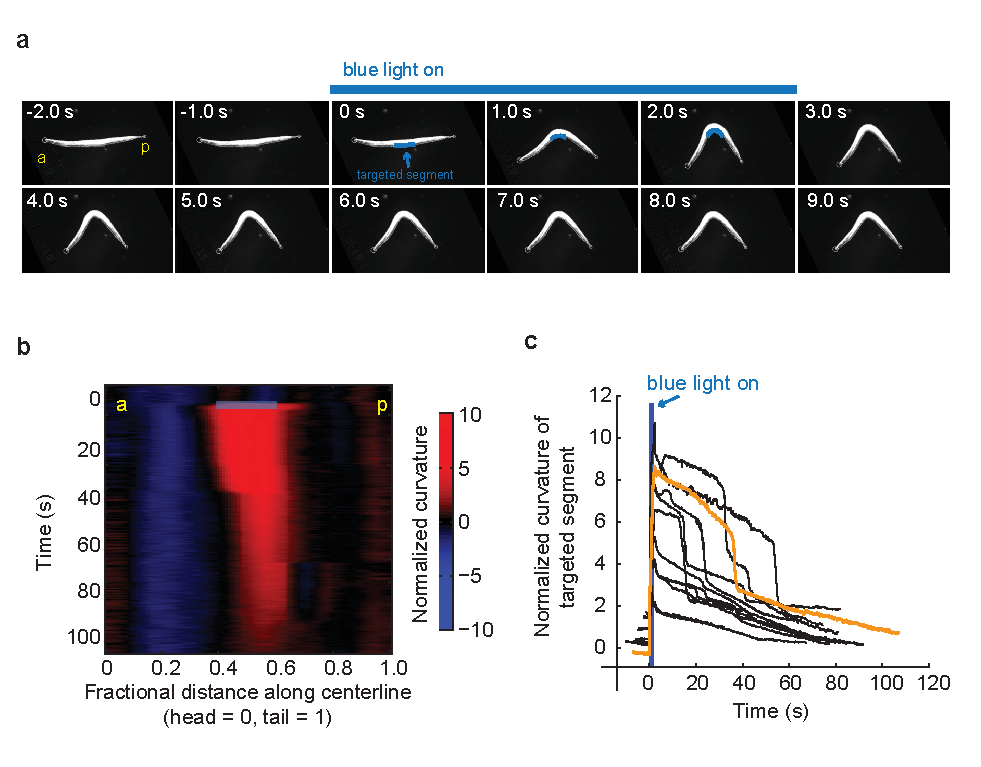
\includegraphics[width=\textwidth]{figures/prop_sup4}
\caption[Muscle hysteresis induced by optogenetic illumination. ] { Muscle hysteresis induced by optogenetic illumination. 
(\textbf{a}) Video images of an ivermectin-treated transgenic worm (P\textit{myo3::ChR2}). In a 2 s interval, 
a targeted rectangular region near the middle of the worm (blue rectangle superposed on video 
images) was illuminated by blue light to induce body bending (also see Video  \ref{video:prop11}). 
(\textbf{b}) Curvature kymograph of the animal shown in (\textbf{a}). White rectangle marks the region and 
duration of blue light illumination. 
(\textbf{c}) Normalized curvature of the targeted region before and after illumination. Data from three 
different worms are shown. Orange data points correspond to the experiment shown in (\textbf{a}) and (\textbf{b}).
\label{fig:prop_sup4}}
\end{figure}




\section{Manuscript Information}
\subsection{Submitted for publication as}
A previous version of this chapter was submitted as \citep{wen_bending_2011}:

\bibentry{wen_bending_2011}

\subsection{The Author's Contribution}
The overwhelming majority of the work in this chapter was performed by Quan Wen. Andrew M.~Leifer assisted with optogenetic experiments and provided technical support regarding instrumentation and experimental design. Additionally, Leifer made major contributions to the analysis software. 

The majority of the manuscript was written by Quan Wen and Aravinthan D.T.~Samuel.
